%\VignetteIndexEntry{The PICS users guide}
%\VignetteDepends{PICS,parallel}
%\VignetteKeywords{Preprocessing, ChIP-Seq, Sequencing}
%\VignettePackage{PICS}
\documentclass[a4paper]{article}
\usepackage{underscore}
\usepackage{hyperref}
%\usepackage{url}
%\usepackage{color, pdfcolmk}
%\usepackage[authoryear,round]{natbib}
%\bibliographystyle{plainnat}


%\newcommand{\scscst}{\scriptscriptstyle}
%\newcommand{\scst}{\scriptstyle}

\title{PICS: Probabilistic Inference for ChIP-Seq}
\author{Xuekui Zhang\footnote{ubcxzhang@gmail.com} and Raphael
  Gottardo\footnote{rgottard@fhcrc.org} and Arnaud Droit\footnote{arnaud.droit@crchuq.ulaval.ca}}

\usepackage{Sweave}
\begin{document}
\maketitle



\textnormal {\normalfont}
A step-by-step guide in the analysis of ChIP-Seq data using the PICS package in R

\tableofcontents
%%%%%%%%%%%%%%%%%%%%%%%%%%%%%%%%%%%%%%%%%%%%%%%%%%%%%%%%%%%%%%%%%%%%%%%%%%%%%%%
\newpage


\section{Licensing}

Under the Artistic license 2.0, you are free to use and redistribute this software. However, if you use this package for your own publication, we would ask you to cite the following paper:

\begin{itemize}
\item[] X. Zhang, G. Robertson, M. Krzywinski, K. Ning, A. Droit, S.Jones and R. Gottardo. (2009). PICS: Pobabilistic Inference for Chip-seq. Biometrics 67, 151-163.
\end{itemize}


\section{Introduction}
ChIP-Seq, which combines chromatin immunoprecipitation with massively parallel
short-read sequencing, can profile in vivo genome-wide transcription
factor-DNA association with higher sensitivity, specificity and spatial
resolution than ChIP-chip. While it presents new opportunities for research,
ChIP-Seq poses new challenges for statistical analysis that derive from the
complexity of the biological systems characterized and the variability and
biases in its digital sequence data. We propose a method called PICS
(Probabilistic Inference for ChIP-Seq) for extracting information from
ChIP-Seq aligned-read data in order to identify regions bound by transcription
factors. PICS identifies enriched regions by modeling local concentrations of
directional reads, and uses DNA fragment length prior information to
discriminate closely adjacent binding events via a Bayesian hierarchical
t-mixture model. Its per-event fragment length estimates also allow it to
remove from analysis regions that have atypical fragment lengths. PICS uses
pre-calculated, whole-genome read mappability profile and a truncated
t-distribution to adjust binding event models to compensate for reads that are
missing due to local genome repetitiveness. PICS estimates uncertainties in
model parameters, and these can be used to define confidence regions on binding event locations and to filter estimates. 

\section{PICS pipeline}
A typical PICS analysis consists of the following steps:
\begin{enumerate}
  \item Convert data to a `GRanges' for efficient processing
  \item Genome segmentation via `segmentPICS'
  \item Estimation of binding site positions and other PICS parameters via `PICS'
  \item Repeat 1-2 by swapping the IP and Control samples
  \item Use 1-3 to estimate the FDR via `picsFDR'
  \item Output enriched regions and `PICS' profiles with bed and wig files
\end{enumerate}

As with any package, you first need to load it with the following command

\begin{Schunk}
\begin{Sinput}
> library(PICS)
\end{Sinput}
\end{Schunk}

\section{Data Input and Formating}
The first step of the PICS pipeline consists of converting the aligned reads (from both IP and control samples) into a format that allows efficient segmentation of the genome into a set of candidate regions that have enough Forward and Reverse reads. The data formatting could be a bed type dataframes as well as `AlignedReads' objects as returned by the function `readAligned' which can read various file formats including Eland, MAQ, Bowtie, etc. Please refer to the `ShortRead' vignette for more details on how to read data into R, other than from a BED file. In the example listed below, we use bed type files, which consists of tab delimited files with the following columns: space, start, end, strand, where each line represent a single read. 

In addition to the IP Control datasets, we use another argument consisting of a mappability profile for the genome interrogated. For each chromosome, a mappability profile for a specific read length consists of a vector of zeros and ones that gives an estimated read mappability `score' for each base pair in the chromosome. A score of one at a position means that we should be able to align a read of that length uniquely at that position, while a score of zero indicates that no read of that length should be uniquely alienable at that position. As noted, reads that cannot be mapped to unique genomic locations are typically discarded. For convenience, and because transitions between mappable and non-mappable regions are typically much shorter than these regions, we compactly summarize each chromosome's mappability profile as a disjoint union of non-mappable intervals that specify only zero-valued profile. We store this information as a bed file where each line correspond a non-mappable intervals. PICS makes use of such mappability profiles to estimate the reads that are missing because they could not be aligned. Mappability profiles for a range of reads lengths and species are available from:

http:/wiki.rglab.org/index.php?title=Public:Mappability_Profile

To make your own mappability profiles, use the script available at:

https://github.com/SRenan/proMap/

Once the data have been read, we can create the `GenomeData' object, which is a list data structure, where each element of the list corresponds to a different chromosome. Each element of the list contains the IP and control reads as well as the mappability profiles for the corresponding chromosome. When reading the data, we can also sort and remove duplicated reads, which is recommended for a PICS analysis (sort is actually required).


In this documentation, the path for the data is:  .../PICS/inst/extdata folder.
\begin{Schunk}
\begin{Sinput}
> path<-system.file("extdata",package="PICS")
> dataIP<-read.table(file.path(path,"Treatment_tags_chr21_sort.bed"),header=TRUE,
+ colClasses=c("factor","integer","integer","factor"))
> dataIP<-as(dataIP,"GRanges")
> dataCont<-read.table(file.path(path,"Input_tags_chr21_sort.bed"),header=TRUE
+ ,colClasses=c("factor","integer","integer","factor"))
> dataCont<-as(dataCont,"GRanges")
\end{Sinput}
\end{Schunk}

\begin{Schunk}
\begin{Sinput}
> map<-read.table(file.path(path,"mapProfileShort"),header=TRUE,
+ colClasses=c("factor","integer","integer","NULL"))
> map<-as(map,"GRanges")
\end{Sinput}
\end{Schunk}


\section{PICS analysis}

\subsection{Genome segmentation}
We segment the genome into candidate regions by pre-processing bidirectional aligned reads data from a single ChIP-Seq experiment to detect candidate regions with a minimum number of forward and reverse reads. These candidate regions will then be processed by PICS. The `minReads' parameter will heavily influence the number of candidate regions returned. In principle, it is better to use a small value for `minReads' in order not to miss any true binding sites. However, a value too small will likely return many false positive regions, which can result a longer computing time for the \texttt{PICS} function.  If a control sample is available you may also chose a value of `minReads' that would give you a ratio of the number of candidate regions in the control over the number of candidate regions in the IP of about 25\%. A ratio larger than 25\% would most likely result in a large FDR when using \texttt{picsFDR}, and therefore it is not necessary to use too low of a threshold. See below for an illustration.  \newline

In order to improve the computational efficiency of the PICS package, we recommend the utilisation of the \texttt{parallel} package, which allows for easy parallel computations. In what follows, we assume that \texttt{parallel} is installed on your machine. If not, you could omit the first line, which will lead a serial execution. By default the command is not run, so you're safe. Note that the \texttt{segmentReads} and \texttt{PICS} functions, will automatically detect whether you have initialized a cluster and if yes it will use it. 

\begin{Schunk}
\begin{Sinput}
> library(parallel)
\end{Sinput}
\end{Schunk}

\begin{Schunk}
\begin{Sinput}
> seg<-segmentPICS(dataIP, dataC=dataCont, map=map, minReads=1)
\end{Sinput}
\end{Schunk}


\subsection{Parameter estimation}
After having segmented the genome into candidate regions, we use the \texttt{PICS} function to detect binding regions in a probabilistic way, and returns binding site estimates, confidence intervals, etc. In the code below, we assume that you are processing transcription factor data, as specified with the `dataType' option set to `TF' for transcription factor. We also plan to support histone modification data in a future release of PICS, which will be turned on by specifying `dataType=`H'. In our case, assuming that we have already segmented the genome using \texttt{segmentReads}, we can proceed with the following command, 

\begin{Schunk}
\begin{Sinput}
> pics<-PICS(seg)
\end{Sinput}
\end{Schunk}

\subsection{FDR estimation}
In order to estimate the FDR, we need to rerun our analysis after swapping the IP and control samples. Note that this requires the presence of a control sample. We proceed with the following commands to compute the FDR after removing binding site estimates with noisy parameters as specify by the filter. 

\begin{Schunk}
\begin{Sinput}
> segC<-segmentPICS(dataCont,dataC=dataIP,map=map,minReads=1)
> picsC<-PICS(segC)
> fdr<-picsFDR(pics,picsC,filter=list(delta=c(50,Inf),se=c(0,50),
+ sigmaSqF=c(0,22500),sigmaSqR=c(0,22500)))
\end{Sinput}
\end{Schunk}

Then once the FDR has been estimated, one can visualize the FDR as a function of the score to pick a threshold that would lead to the desired FDR. 

\begin{Schunk}
\begin{Sinput}
> plot(pics,picsC,xlim=c(2,8),ylim=c(0,.2),filter=list(delta=c(50,300),
+ se=c(0,50),sigmaSqF=c(0,22500),sigmaSqR=c(0,22500)),type="l")
\end{Sinput}
\end{Schunk}
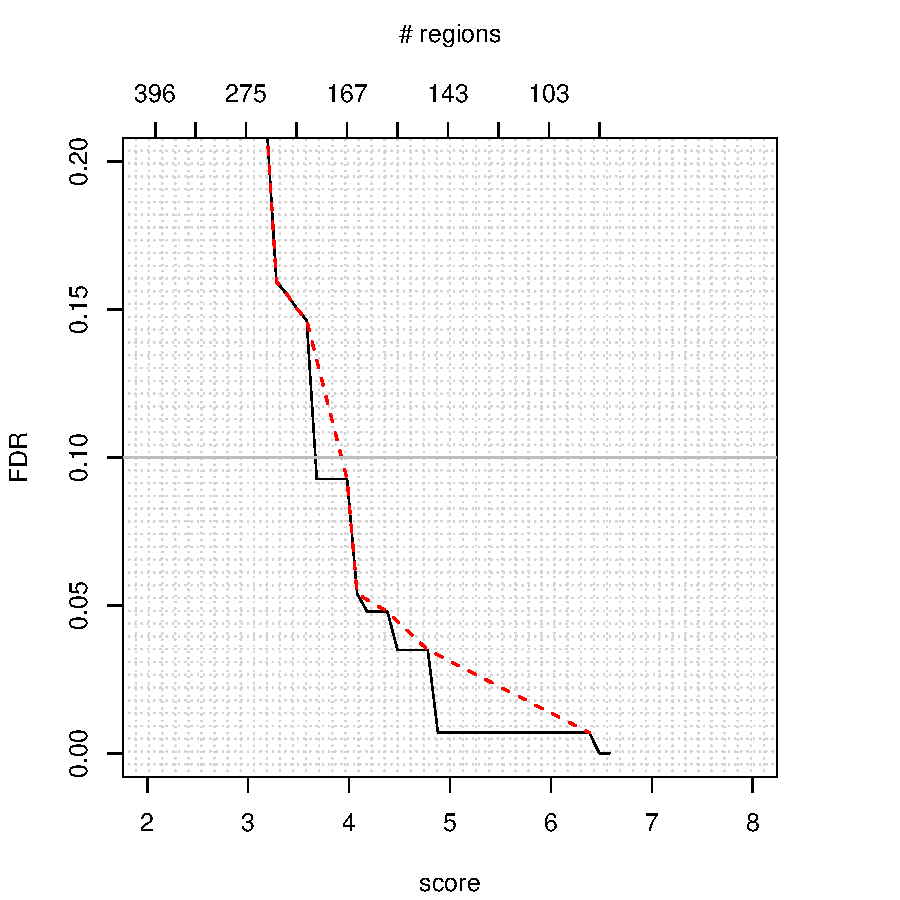
\includegraphics{PICS-plot-FDR1}

You can also visualize the FDR as a function of the number of regions.

\begin{Schunk}
\begin{Sinput}
> plot(fdr[,c(3,1)])
\end{Sinput}
\end{Schunk}
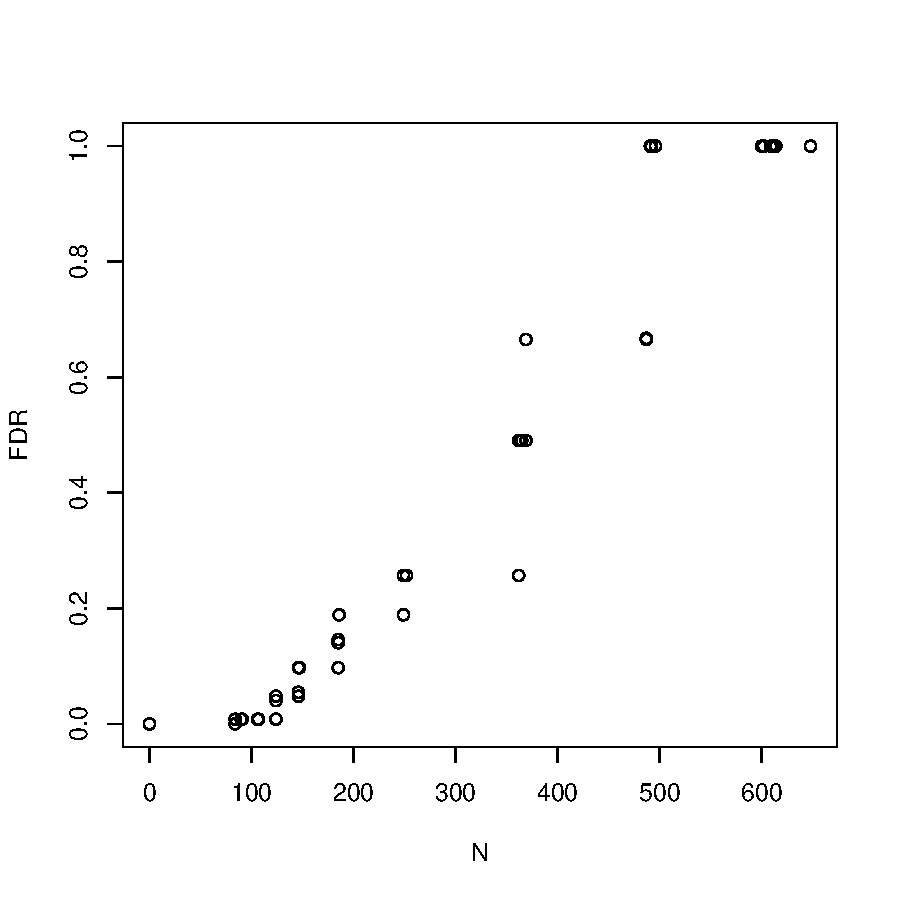
\includegraphics{PICS-plot-FDR2}

\section{Result output}

To facilitate data processing and data output, we make use of the \texttt{IRanges} package to summarize our results as `RangedData' objects. The resulting `RangedData' objects can then be analyzed with the \texttt{IRanges} package and/or exported to bed/wig files with the \texttt{rtracklayer} package. In each case, we can make use of filters noisy regions and or regions with too low of score. In particular the \texttt{picsFDR} function can be used to set the score threshold leading to the desired `FDR'.

\subsection{Writing enriched regions to BED files}

\begin{Schunk}
\begin{Sinput}
> myFilter=list(delta=c(50,300),se=c(0,50),sigmaSqF=c(0,22500),sigmaSqR=c(0,22500))
> rdBed<-makeRangedDataOutput(pics,type="bed",filter=c(myFilter,list(score=c(1,Inf))))
\end{Sinput}
\end{Schunk}
The following command will create the appropriate bed files, and because it requires the \texttt{rtracklayer} package, we do not run it here but simply displayed for your purpose.
\begin{Schunk}
\begin{Sinput}
> library(rtracklayer)
> export(rdBed,"myfile.bed")
\end{Sinput}
\end{Schunk}

\subsection{Writing density scores to WIG files}
The following command will create the appropriate `RangedData' and corresponding wig file, and because it requires the \texttt{rtracklayer} package, we do not run it here but simply displayed for your purpose.

\begin{Schunk}
\begin{Sinput}
> rdBed<-makeRangedDataOutput(pics,type="wig",filter=c(myFilter,list(score=c(1,Inf))))
> export(rdBed,"myfile.wig")
\end{Sinput}
\end{Schunk}


\end{document}

